% !TEX program = xelatex
\documentclass[11pt]{article}
\usepackage[margin=1in]{geometry}
\usepackage{nopageno} % no page numbers

\usepackage{graphicx}
\graphicspath{ {./graphics/} }
\usepackage[dvipsnames]{xcolor}
\definecolor{CrispBlue}{HTML}{0176AE}

\usepackage{fontspec}
\usepackage{tcolorbox}
\usepackage{etoolbox}
\BeforeBeginEnvironment{verbatim*}{\begin{tcolorbox}[colback=CrispBlue!5!white,colframe=CrispBlue!75!black]}%
\AfterEndEnvironment{verbatim*}{\end{tcolorbox}}%


\usepackage{hyperref}
\hypersetup{
    colorlinks,
    citecolor=black,
    filecolor=black,
    linkcolor=black,
    urlcolor=black
}

\usepackage{subcaption}
\setlength{\parindent}{0pt}
\setlength{\parskip}{1em}

\usepackage{tocloft}
\renewcommand{\cftpartleader}{\cftdotfill{\cftdotsep}}
\renewcommand{\cftsecleader}{\cftdotfill{\cftdotsep}}

\usepackage{fancyhdr}
\pagestyle{fancy}
\fancyhf{}
\lhead{ECE 517: Machine Learning}
\rhead{Assignment 3.2}
\rfoot{Page \thepage}

\usepackage{amsmath,amsfonts,amssymb}
\usepackage{bm}
\usepackage{mathtools}

\renewcommand{\listfigurename}{List of Figures}

\begin{document}
\setmainfont{SF Pro Text}
\setsansfont{SF Pro Text}
\setmonofont{SF Mono}
\renewcommand{\familydefault}{\sfdefault}


\thispagestyle{empty}
\begin{titlepage}
\vspace*{\fill}
\begin{center}
\textsc{\Huge{ECE 517: Machine Learning}}\\[3em]
\textsc{\LARGE Assignment 3.2: LIBSVM Experiments}\\[6em]
\textsc{\Large David Kirby -- 101652098 -- davidkirby@unm.edu}\\[3em]
\textsc{\Large Fall 2021}
\end{center}
\vfill
\begin{figure}[h]
\begin{subfigure}{0.5\textwidth}

\includegraphics[width=0.25\linewidth]{learning.png}
\end{subfigure}
\begin{subfigure}{0.6\textwidth}\hspace{1em}

\includegraphics[width=0.8\linewidth]{new-soe-logo.png}
\end{subfigure}
\end{figure}
\end{titlepage}
\setcounter{figure}{0}

\hypersetup{
    linkcolor=CrispBlue,
    urlcolor=CrispBlue,
    breaklinks=true
}

This assignment is intended to construct a Support vector machine using standard software. You can use MATLAB or Python to completer this assignment.

The link to download the software is here: \hyperlink{https://www.csie.ntu.edu.tw/~cjlin/libsvm/}{SVM-LIB}. You will need to download, expand and install the software in a folder. If you use MATLAB, you will need to add the corresponding folder to the path. If you use Python, you will find the corresponding libraries in the folder.

For Windows users, find the subdirectory ``Windows'' with precompiled files, that can be called by MATLAB. If they do not work with your Windows version, go to the subdirectory ``MATLAB'', and there you will find C files that you will need to compile from MATLAB. Just type ``make'' from MATLAB. Then use the complied executable files.

Please find instructions on how to use the functions ``svmtrain'' and ``svmpredict'' in the assignment file below and the videos.

\begin{tcolorbox}[colback=CrispBlue!5!white,colframe=CrispBlue!75!black,title=3.1 Construction of a classifier with the model parameters.]
Using the parameters of the training, construct a machine that classifies the training data. Compare your results with the ones of \texttt{svmpredict}. In order to find the equation of the classifier, you must compute the primal parameter \( \bm{\mathrm{x}} \) from the dual ones \( \alpha_i \) and the data.
\end{tcolorbox}
\begin{figure}[h]
    \begin{subfigure}{0.5\textwidth}
    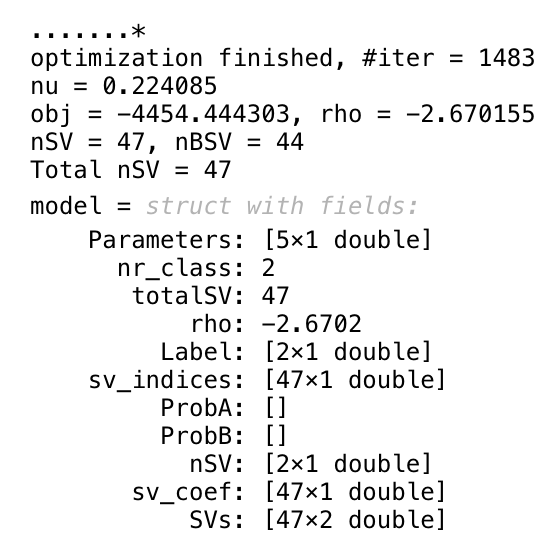
\includegraphics[width=0.8\linewidth]{modelParam.png}
    \caption{Construction of classifier.}
    \label{fig:Param}
    \end{subfigure}
    \begin{subfigure}{0.6\textwidth}\hspace{1em}
    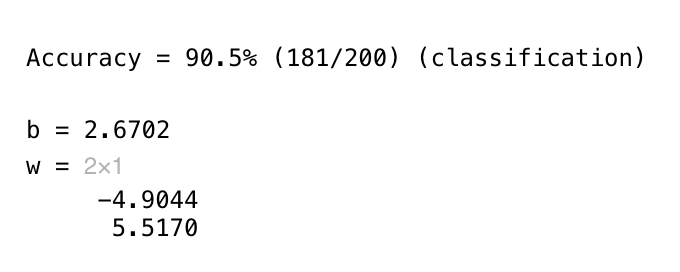
\includegraphics[width=0.8\linewidth]{svmpredict.png}
    \vspace{8.8em}\caption{Comparison with \texttt{svmpredict}.}
    \label{fig:svmPredict}
    \end{subfigure}
\end{figure}
\newpage
\begin{tcolorbox}[colback=CrispBlue!5!white,colframe=CrispBlue!75!black,title=3.2 Graphical representation of an SVM.]
Use the example of subsection 2.1 to plot the separating line, the two margin lines and the support vectors resulting of the SVM training. Do it for a smaller value and a higher value of parameter `sigma' of the data generating code. Comment the results.
\end{tcolorbox}

\begin{figure}[ht]
    \centering
    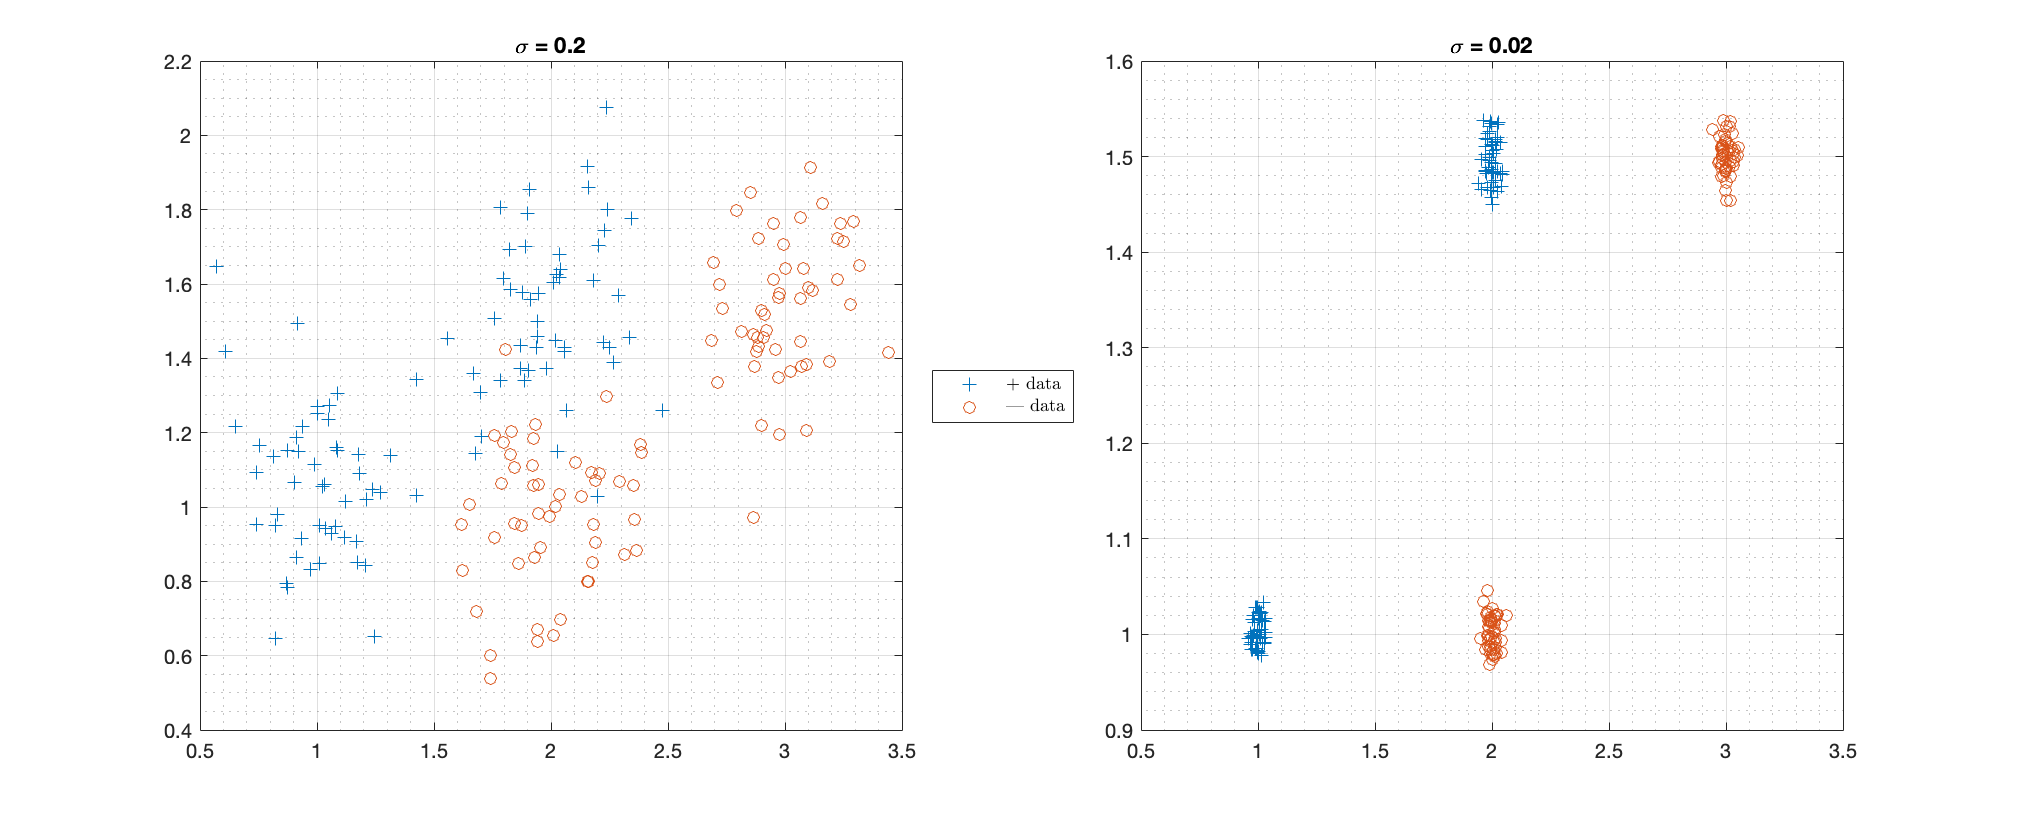
\includegraphics[width=\textwidth]{sampleData.png}
    \vspace{-1em}\caption{Datapoints with \( \sigma = 0.2\) and \( \sigma = 0.02 \).}
    \label{fig:sampleData}
\end{figure}

\begin{figure}[ht]
    \centering
    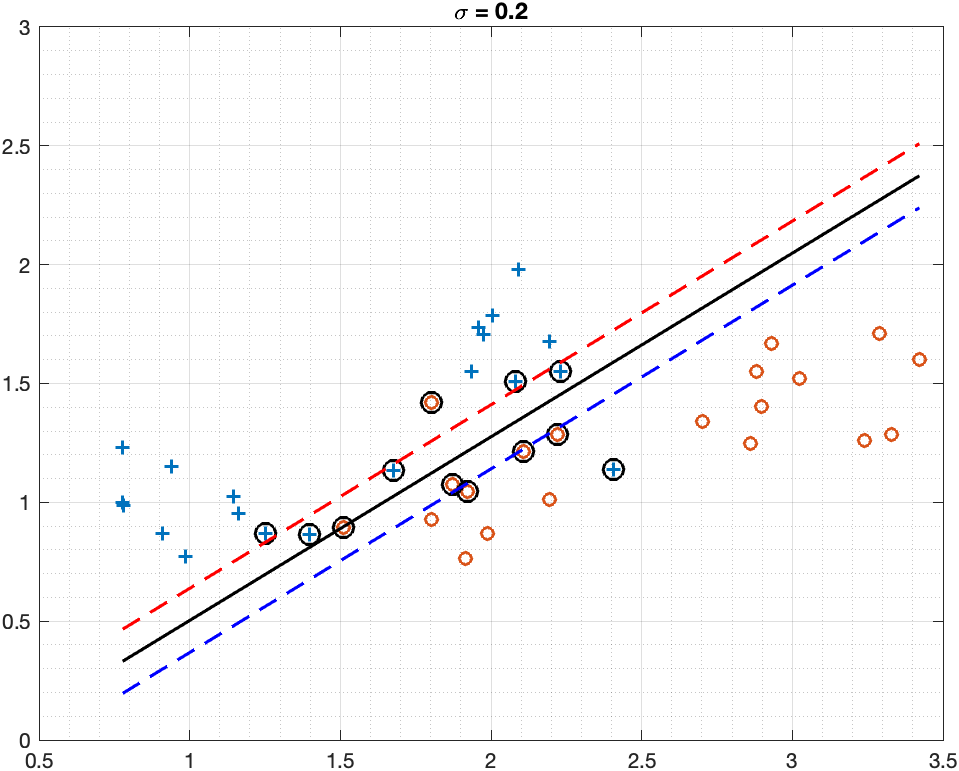
\includegraphics[width=\textwidth]{SVM_sig0.2.png}
    \vspace{-1em}\caption{Support vectors for \( \sigma = 0.2\).}
    \label{fig:SVM-0.2}
\end{figure}

\begin{figure}[ht]
    \centering
    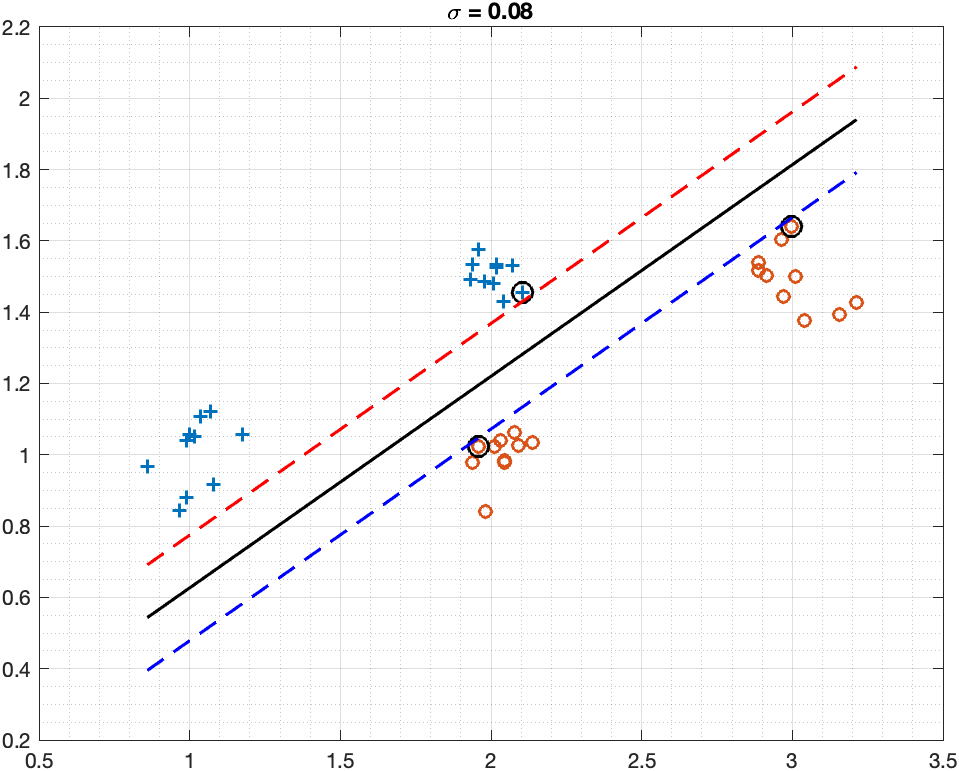
\includegraphics[width=\textwidth]{SVM_sig0.08.png}
    \vspace{-1em}\caption{Support-vectors for \( \sigma = 0.08\).}
    \label{fig:SVM-0.08}
\end{figure}

\begin{tcolorbox}[colback=CrispBlue!5!white,colframe=CrispBlue!75!black,title=Comments]
    To better see what was happening when plotting, I increased \(N\) from 10 to 50. I also chose to vary \( \sigma \) from 0.2 to 0.08 to get a better idea for what is being changed. As is evidenced by the plots in Figure~\ref{fig:sampleData}, \( \sigma \) determines how separated the data is from the center. To this end, we can think of \( \sigma \) as the standard deviation.
\end{tcolorbox}
\clearpage
\begin{tcolorbox}[colback=CrispBlue!5!white,colframe=CrispBlue!75!black,title=3.3 Estimating the structural risk.]
The objective of this exercise is to draw a plot of the actual risk ($R(\alpha )$) and the empirical risk $R_{emp} (\alpha )$. Consider a space of 10 dimensions and a set of data that can be represented and classified in a subspace of only 3 dimensions. Thus, a linear classifier of $h=4$ should be sufficient to properly solve the classification problem.
\end{tcolorbox}

\begin{figure}[ht]
    \centering
    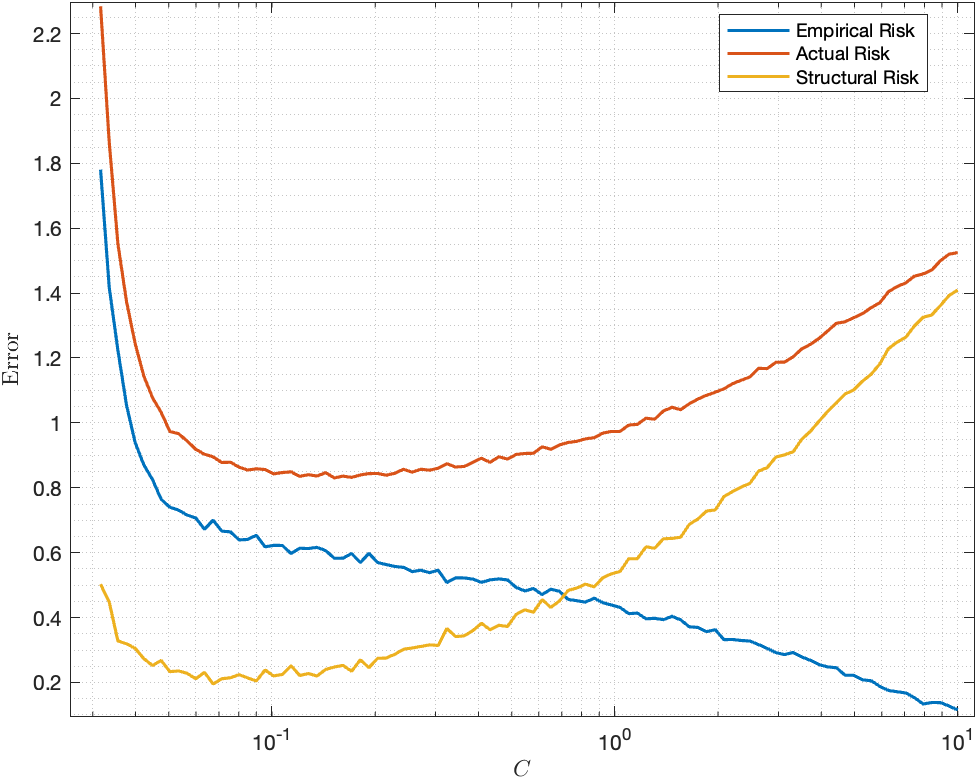
\includegraphics[width=\textwidth]{Risk.png}
    \vspace{-1em}\caption{Plot of actual, empirical, and structural risks.}
    \label{fig:Risks}
\end{figure}

\end{document}